\section{Introduction}
Carbonic anhydrase (CA) catalyzes the interconversion of carbon dioxide and carbonic acid/bicarbonate as follows:
\begin{align}\label{eqn:ca_reaction}
\ce{CO_2 + H_2O 
<=>[\ce{CA}] 
H_2CO_3}
\end{align}
CA relies on a \ce{Zn^2+} cofactor for its catalytic activity. The zinc ion can be stripped from the enzyme using a lewis base ligand, which donates electrons to the ion to form a covalent bond. The ligand being studied in this experiment is 2,6-pyridinecarboxylate, commonly called dipicolinate (or dipic). Figure \ref{fig:dipic} shows the structure of dipic. In this experiment, the rate of zinc removal by dipic will be measured.
\begin{figure}[h]
  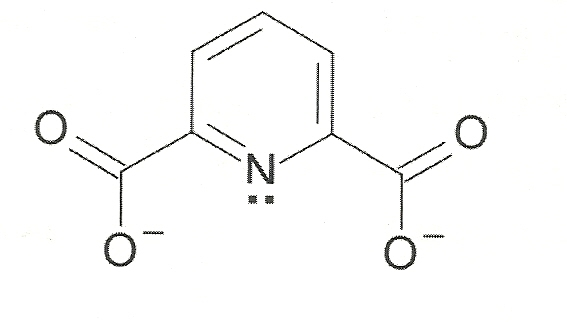
\includegraphics[scale=0.5]{./Figures/dipic.jpg}\\
  \caption{Structure of 2,6-pyridinecarboxylate (dipic)}\label{fig:dipic}
\end{figure}
 